\section{Rappel des fonctionnalités de la solution informatique et organisationnelle}

Une solution standard est une solution qui s’appuie sur les bonnes pratiques recommandées par un éditeur de progiciel de gestion intégré. L’information est mise à jour en temps réel dans l’ensemble des modules associés au module qui vient d’être modifié, et il est aisé de retrouver l’origine de chaque information. Cette solution peut couvrir l’ensemble du SI d’une entreprise, ou bien seulement une partie si l’on choisit de n’implémenter que certains modules de SAP. \\

Pour SPIE, nous avons choisi l’ERP SAP, et celui-ci couvrira l’ensemble du SI lié aux métiers de la maintenance. Le choix de cette solution permettrait d’homogénéiser le SI de SPIE avec un outil unique couvrant un très large périmètre de gestion. La découpe en modules fonctionnels permet une personnalisation maximale, chacun couvrant un des périmètres de l’entreprise.

\section{Chiffrages des coûts (d'acquisition et de possession)}

\begin{shaded}
\noindent\textsc{Note :} 

Voir Annexe A pour le tableau d'évaluation.
\end{shaded}

Il y a deux types de coûts : les coûts d’acquisition et les coûts de possession. Les premiers ne seront investis qu’une seule et unique fois par l’entreprise, tandis que les seconds permettent le fonctionnement de la société et permettent d’exploiter les biens acquis précédemment. \\

En faisant le choix d’une solution standard, appuyée sur SAP, les coûts d’acquisition sont assez minimes. En effet, les investissements sur cette solution sont peu portées sur les immobilisations corporelles, telles les tablettes tactiles, mais plus sur un coût de formation SAP, délivré aux employés de SPIE Sud-Est. \\

Cependant, si l’investissement initial est peu élevé, la majorité des coûts de la solution standard seront répartis dans le temps. En effet, SAP By Design fonctionne sur un système d’abonnement : pour chaque utilisateur, et chaque année, un abonnement de 1 596 euros doit être payé. Certains services sont également payant, proportionnellement au prix de l’abonnement, par un ratio de 1. Étant donné le nombre important d’utilisateurs de la solution, soit 300 techniciens et 20 utilisateurs sur site, il est compréhensible que les coûts montent rapidement. En revanche, les coûts de maintenance, liés à l’investissement initial correspondant à un pourcentage de ce dernier, ne représentent pas un important montant annuel. La deuxième source de coût de possession correspond aux salaires des nouveaux poste de travail suggérés pour superviser les nouveaux équipements proposés.


\begin{figure}[H]
    \noindent\makebox[\textwidth]{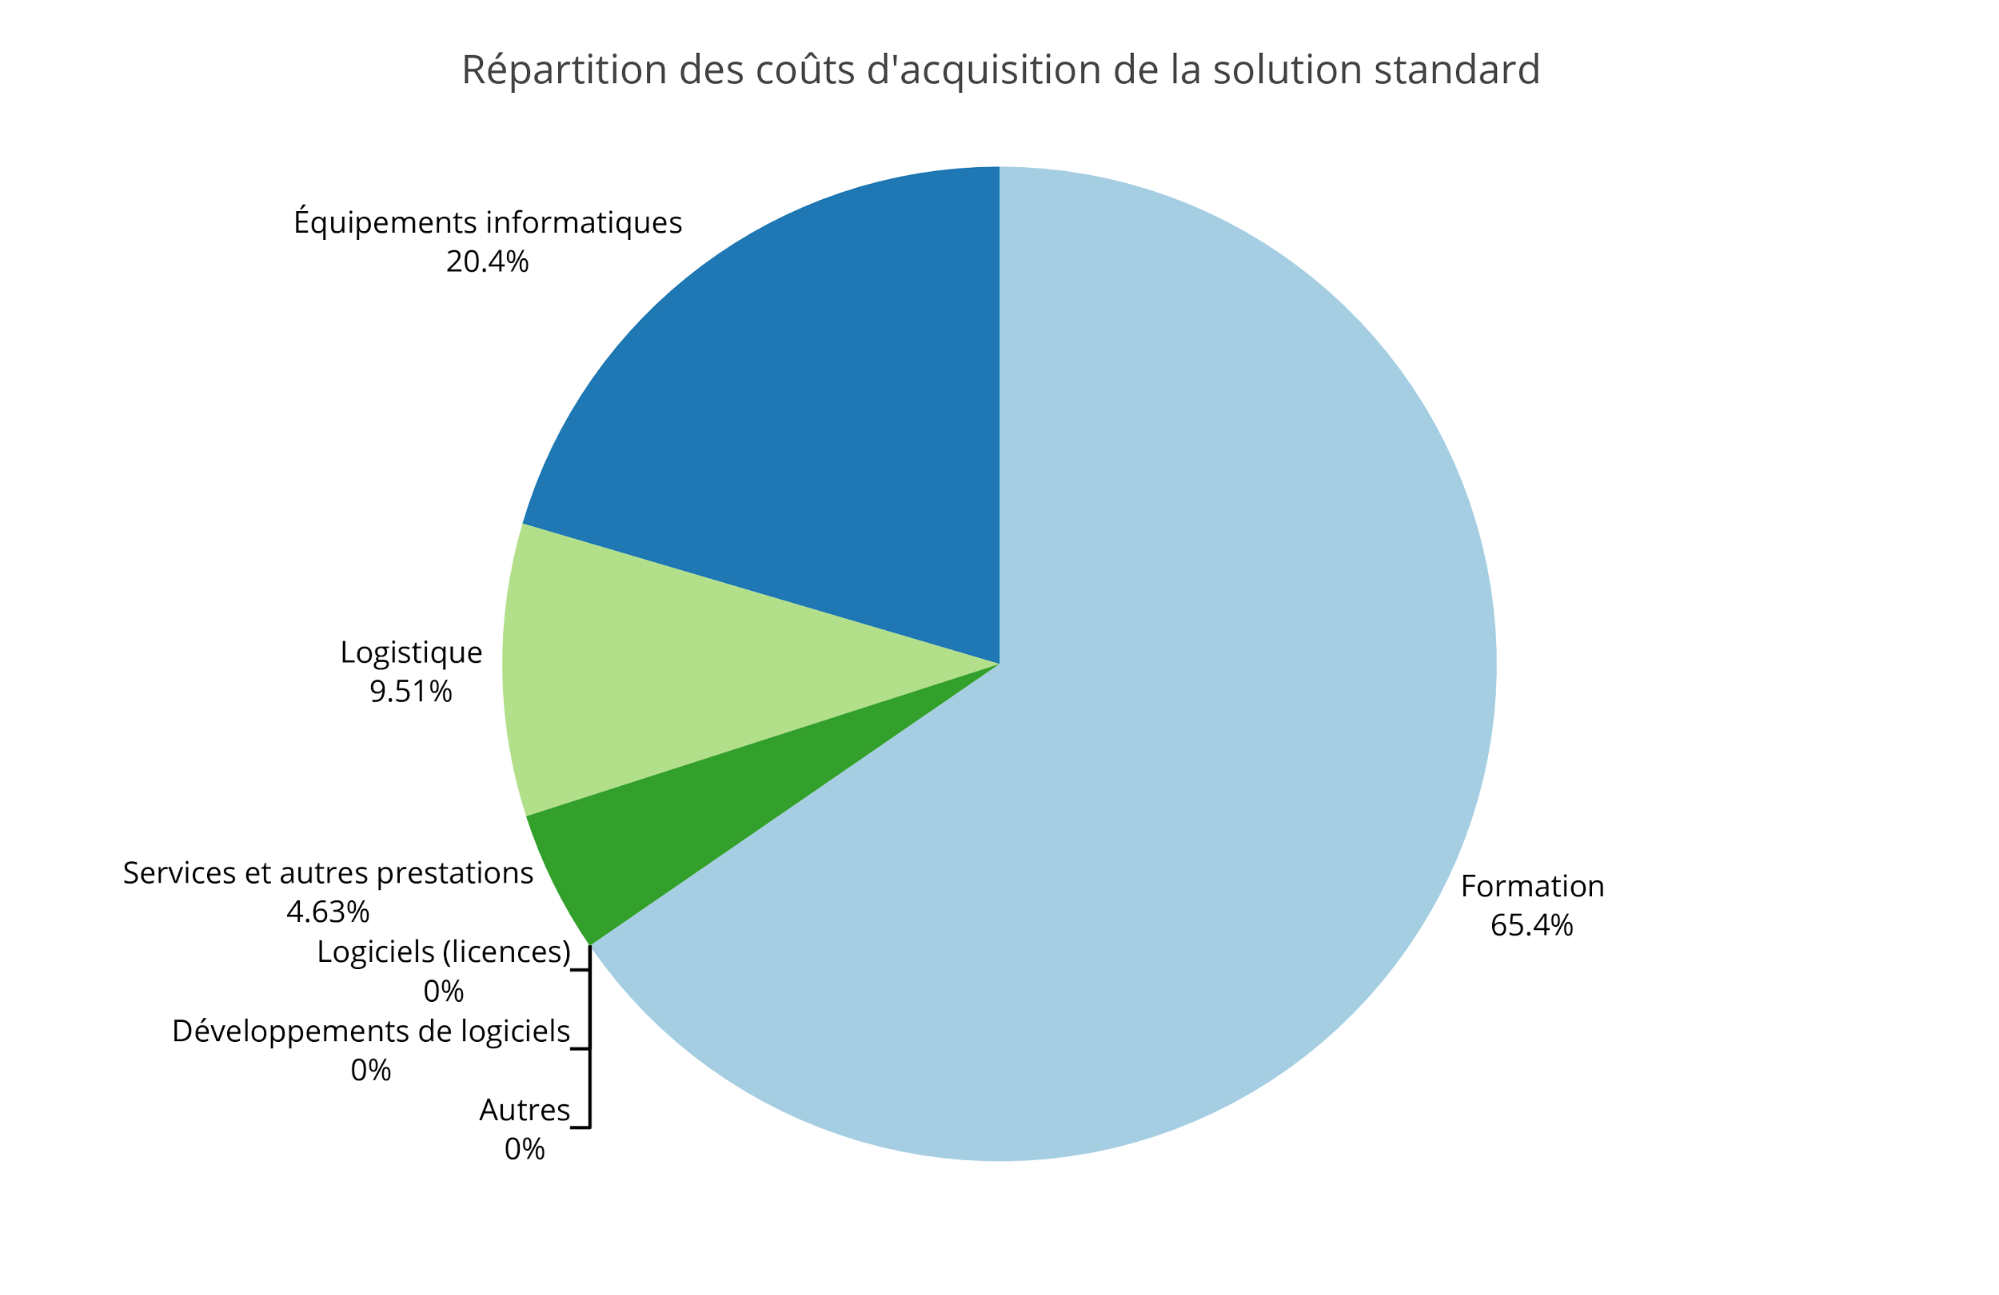
\includegraphics[width=12cm]{figures/cout_acquisition_sol_standard.png}}
\end{figure}

\begin{figure}[H]
    \noindent\makebox[\textwidth]{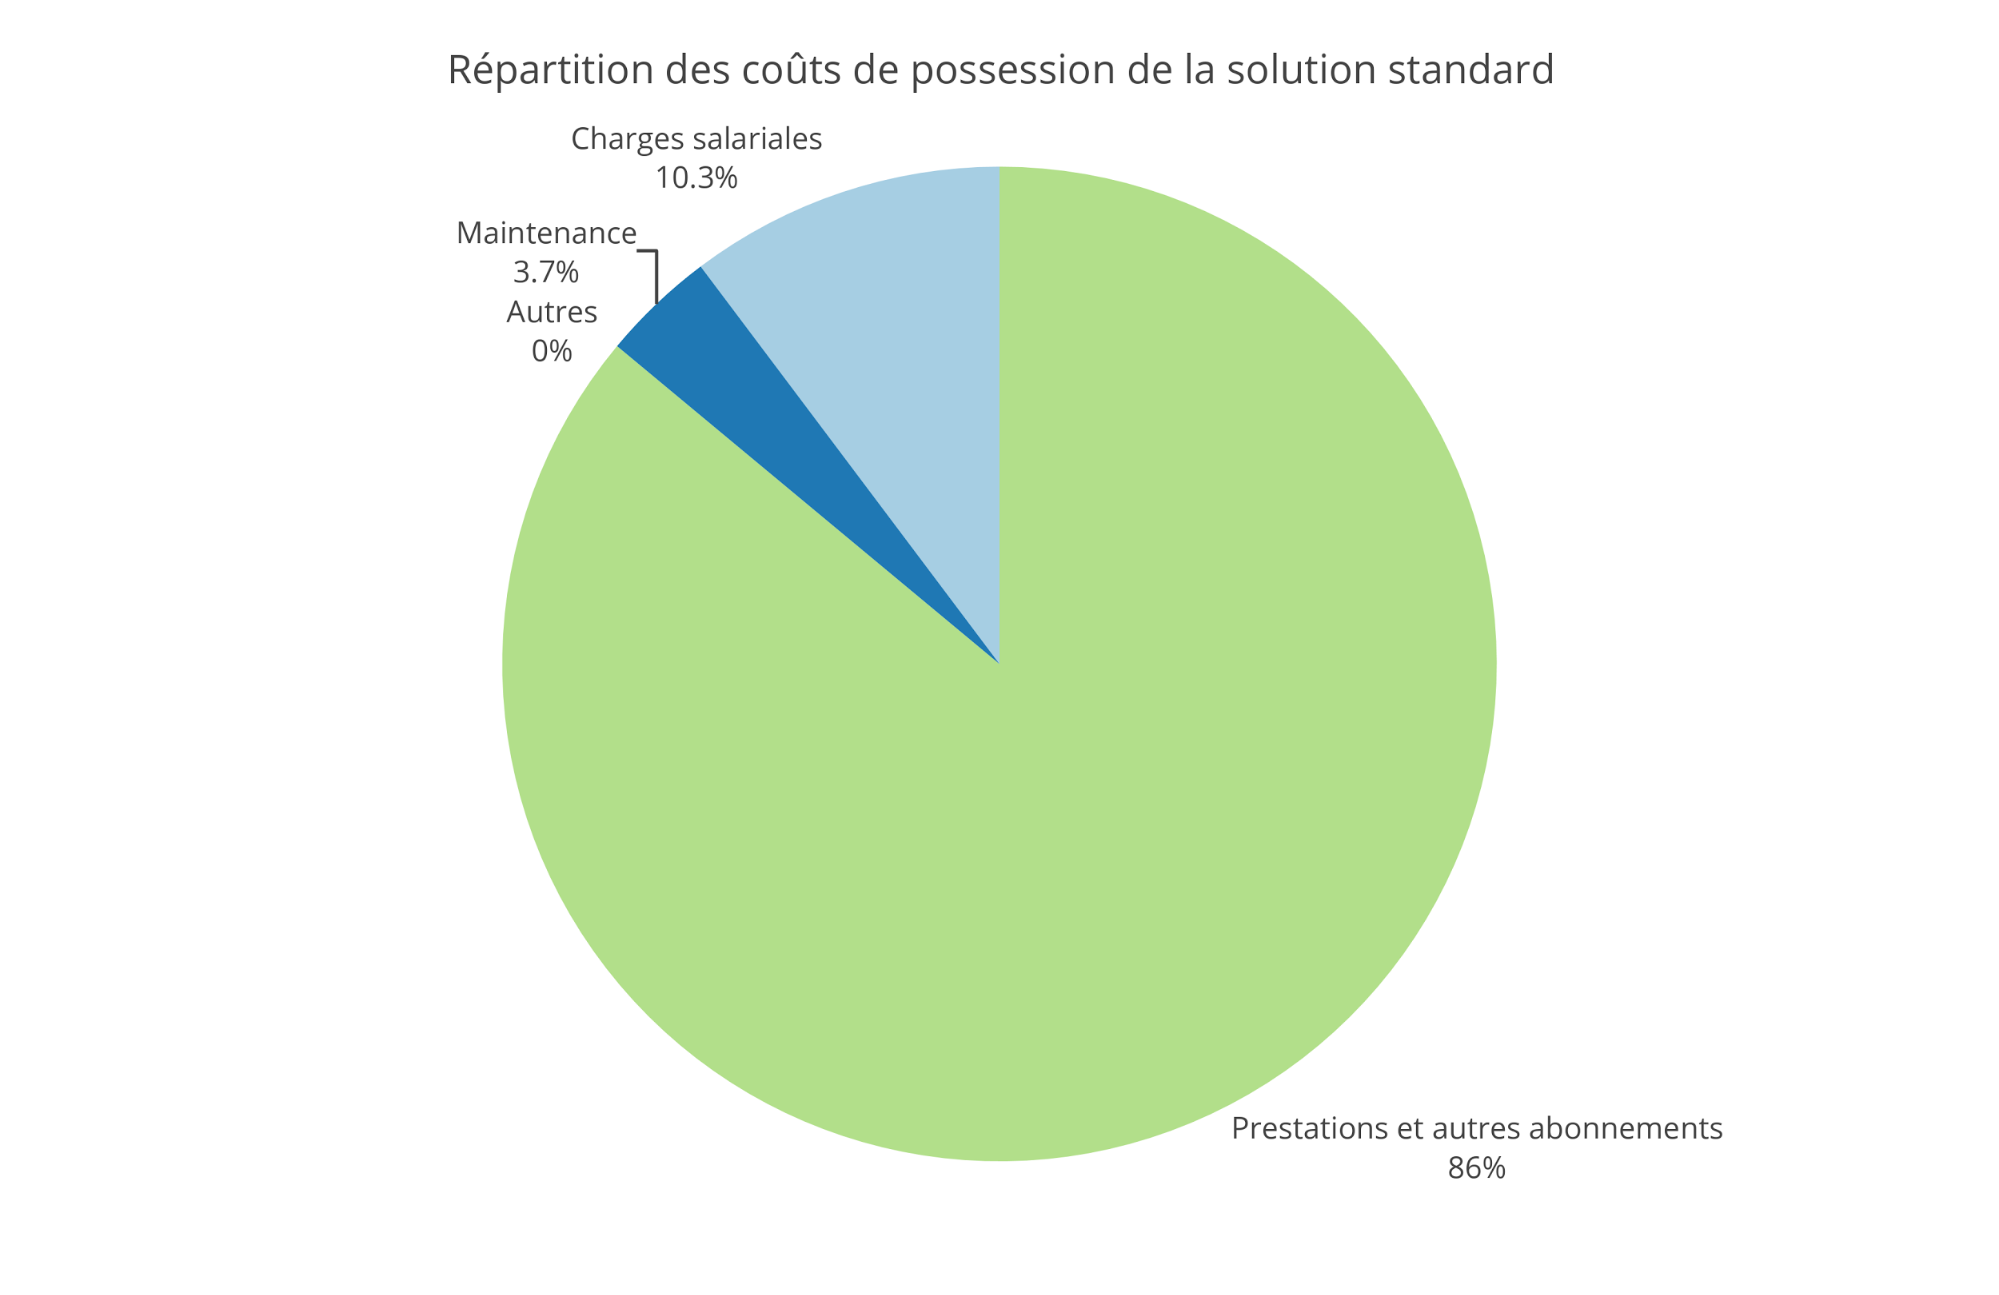
\includegraphics[width=12cm]{figures/cout_possession_sol_standard.png}}
\end{figure}


\section{Retour sur investissement (gains)}

\begin{shaded}
\noindent\textsc{Note :} 

Voir Annexe A pour le tableau d'évaluation.
\end{shaded}

Cette solution permettrait de nombreuses améliorations au sein du fonctionnement de l’entreprise. En effet, en passant par une solution standard, les coûts de maintenance sont fortement réduits. Cette réduction a un impact à la fois sur la maintenance logicielle et d’infrastructure. Des économies sont ainsi réalisées sur la réduction du nombre de jours de développement nécessaires et sur la réduction du nombre de jours soumis aux pannes matérielles, logicielles et réseau. De plus, grâce à la mise à disposition d’une plateforme optimisée et un suivi des processus amélioré, la productivité des employés s’en trouve grandement améliorée, permettant ainsi d’estimer de potentiels gains annuels. \\

En considérant la somme des gains réalisée chaque année grâce à cette solution standard et en intégrant les coûts de possession annuels, nous obtenons un retour sur investissement de 435 752 euros, par an. Ce retour sur investissement permet de rendre cette solution rentable en 10 mois, après sa mise en place.

\section{Évaluation des autres critères de comparaison}

Le fait d’utiliser la solution standard présente d’autres avantages. En effet, la solution sera déployée très rapidement et une transition plus rapide est possible. Il est bien connu que les périodes de transition ne sont pas favorables à une meilleure productivité. C’est dans ce cadre là que la solution standard a un atout certain car pas d’attente de réalisation très longue.

SAP est également pensé pour l’évotutivité et permet une rétrocompatibilité forte. C’est un avantage certains par rapport à d’autres ERP que l’on trouve sur le marché. Ainsi, par exemple l’ERP open-source \bf{odoo} peut demander une mise à jour complète de la base de donnée lors d’un changement de version.

On peut également supposer que de part l’importante utilisation de SAP dans le monde, la sécurité du logiciel est assez bien conçue. Cependant des recherches sur des moteurs de recherches en ligne avec pour mots clefs “failles SAP” montrent que le logiciel est quand même assez souvent victime de failles et de bugs. Ceci est également un des défauts de sa large utilisation. En effet, plus un logiciel est utilisé et plus il peut très intéressant de trouver de d’exploiter d’éventuelles failles.

La dernière chose à souligner dans  le cas de la solution standard est l’installation. Celle-ci n’est pas forcément aisée à faire manuellement. De ce fait il faudra l’intervention d’un consultant SAP pour l’installation, ainsi éventuellement d’un consultant de PeopleSoft de manière à ce que les différents logiciels interagissent correctement.